\section{Integration test}

In order to test that our components interact together according to the specifications, we have chosen to perform integration testing of the system.

Integration testing has the purpose of testing that two units work together. 
Traditionally, integration testing is done by integrating two modules at a time, either from the top of the dependency tree or from the bottom.
There exists a variant, in which the whole system is tested together, instead of pair-wise, called big bang integration testing.
We have chosen to perform our test with this method, due to time limitations \cite{inttest}.

\subsection{Test setup}
The purpose of the tests we have designed is to check if the system can produce sensible predictions for the bikes in the system.

In order to generate test data, we have created a method for simulating real world data. 
The simulator gets a list of destinations (in the form of addresses) as input, making it possible to adjust the probability of the system, by deliberately choosing certain destinations.
This makes it possible to create a data set, where it is possible to predict the expected result.
\stefan{\mikkel{Jeg synes ikke det er helt tydeligt at man kan sætte probability for enkelte adresser. ''adjust the probability of the system''}}

\paragraph{What to test}
We want to test if the system works as specified in the problem statement.
The problems we want to focus on in testing are \ref{pr_few}: \textit{Too few stations} and \ref{pr_arrive}: \textit{No way of knowing when a bike will arrive}. 
The full problem statement can be found in \cref{problem_statement}.
We want to test the following parts of our system in order to test the two problem statement items:

\begin{itemize}
\item Finding hotspots 
\item Markov Chains
\end{itemize}

We test the hotspot creation in order to check if hotspots are generated where there is bike activity, and this to check if the created hotspots will work as a stand in for the old stations.
\stefan{\mikkel{''and this to check''}}
This corresponds to item \ref{pr_few} in the problem statement.

We test the Markov chains in order to figure out if our method of generating Markov chains give proper values for using when predicting the behavior of the bikes.
This corresponds to item \ref{pr_arrive} in the problem statement.

\subsection{Finding hotspots}
All predictions are calculated based on the generated hotspots.
Misplaced hotspots can therefore skew the results, decreasing the precision of the predictions.
Thus, we want to test whether or not the hotspots are generated as expected.

\paragraph{Test data}
For this test, we have constructed a data set, which consists of two addresses:
\begin{itemize}
\item Nytorv 1, 9000 Aalborg
\item Nytorv 15, 9000 Aalborg
\end{itemize}
and their corresponding GPS coordinates.
We will then generate hotspots based on this data, and compare the center of these hotspots, with the addresses from the constructed data set.
Because the addresses are the only place where the bikes stand still, and the data is generated with noise there should only be clusters around these addresses.
\mikkel{Hvorfor er støj en grund til at der kun laves clusters på de adresser?}
\mikkel{WORKWORK: Der er støj - derfor bliver clusters større end 1 punkt.}

\paragraph{DBSCAN parameters}
The clustering algorithm chosen\footnote{DBSCAN explained in \Cref{clustering:DBSCAN}} expects two parameters, $eps$ and $MinPts$.
Because real data is not available the chosen values for the parameters are based on the following.

The $MinPts$ parameter was set to 4 as suggested by \citet[Page 529]{pang2006introduction}.
For the other parameter, $eps$, 15 meters was chosen.
This value was chosen because a GPS receivers accuracy is 15 meters according to \citet{garmingps}.
Setting $eps \leftarrow 15$ makes sense because a GPS data point then can be up to 15 meters away from its real location.
\mikael{Argumenter for at det giver mening ift. test da vi regner med at ramme samme punkt}

\paragraph{Result}
The result has been visualized and can be seen in \Cref{fig:test:clustering}.
The figure shows as expected, two hotspots and a path of GPS data points in-between.
The test verifies that all GPS data points, that should be in a hotspot, actually are (as illustrated by the circles in \Cref{fig:test:clustering}).
This means that the clustering is accurate and works as expected.
One should keep in mind that the DBSCAN parameters, which worked with the constructed data set, may need to be calibrated when used on real data.

\begin{figure}
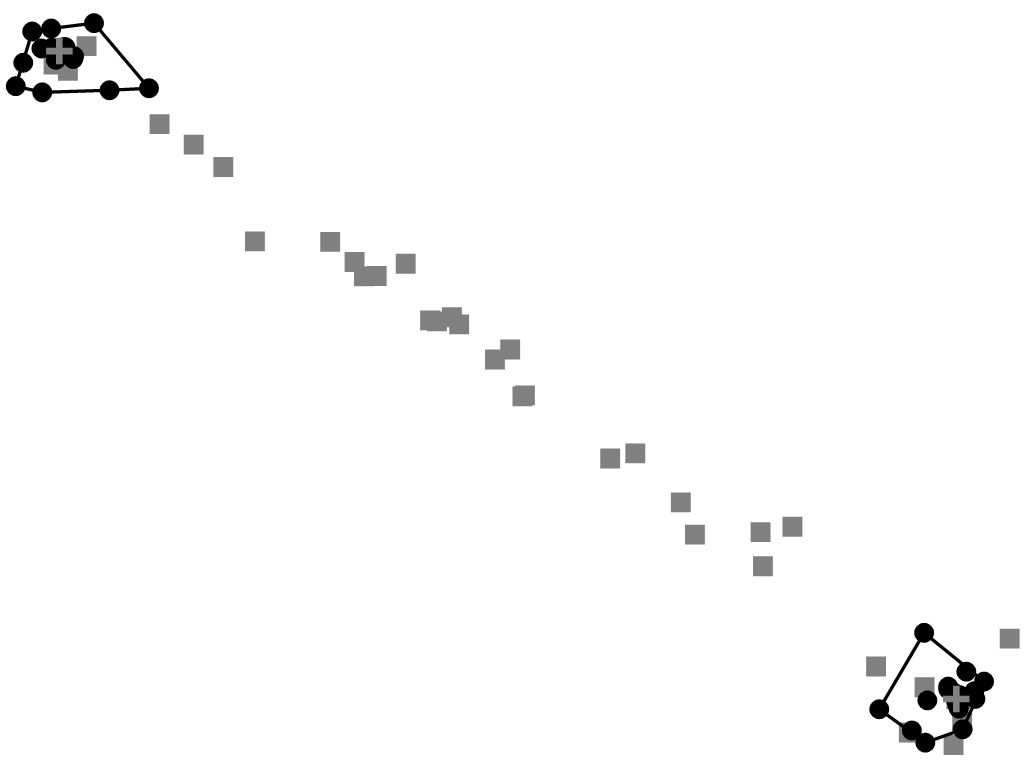
\includegraphics[width=\textwidth]{clusteringTest}
\caption{The clustering test results. 
The crosses indicating the coordinates of the two given addresses. The squares representing GPS points received while a bike is moving. The circles representing when a bike stands still. The line connecting the circles is the cluster represented by a polygon(a hotspot).}
 Keep in mind that the squares inside a cluster are not part of a cluster.
\label{fig:test:clustering}
\end{figure}

\subsection{Predictions}
The users rely on the predictions of bike usage, as stated in \Cref{prob_statement:solution}, item 5.
It is therefore important to test how well the predictions work.

\paragraph{Test data} To test this we create a number of controlled data sets.
The data sets are controlled by assigning probabilities of choosing the destinations. 
We then know where to expect the probabilities to be high.

The data is constructed in such a way that every time a bike arrives at a hotspot it will wait for 12 minutes, before going to the next destination.
This ensures that there is registered at least two points within a hotspot.

The addresses are placed in such a way that it should not be possible to go from one hotspot to another in a single update interval.
This means that it should only be possible to get to a hotspot from a departure state, and not directly.
This means that every hotspot row in the result should contain only two numbers, the transition to itself and the transition to its departure state.

In order to display results, tables depicting the generated Markov Chain matrix are displayed.
$h$ indicates a hotspot while $d$ indicates a departure state.
The number in $ (d_1,h_2) $ indicates the probability in percentages of transitioning from departure state 1 to hotspot 2. 

\subsubsection{Even distribution}
The simplest test case is when the generated data has equal probability of choosing every destination. 
In this case we would expect the probabilities of a bike arriving at every destination to be the same.

The data was generated to simulate a 15 hour period with 100 bikes and 4 possible addresses:
\begin{itemize}
\item Nørresundby Torv, 9400 Nørresundby
\item Nytorv, 9000 Aalborg
\item Borgmester Jørgensens Vej 5, 9000 Aalborg
\item Selma Lagerløfs Vej 300, 9220 Aalborg Ø
\end{itemize}
The results for the test can be seen in \Cref{test_even}.

In the result it is seen that some inaccuracies have occurred since there are some entries with values that, although very low, are not zero as expected.
\mikkel{WORKWORK: Vi mangler et eksempel på sådan en værdi.}

The important numbers are those that tell how a bike act when in a departure state.
These are the numbers that indicate how the routes are expected to be chosen.
These numbers are setwise marked with a color in the table.

Each of these sets of numbers indicate the distribution between destinations.
As the distribution of the generated data was set to be equal, we would expect these numbers to be equal as well.

\begin{figure}
	\centering
\begin{tabular}{|c | c c c c c c c c|}
\hline
\% &      $ h_1 $ & $ d_1 $ & $ h_2 $ & $ d_2 $ & $ h_3 $ & $ d_3 $ & $ h_4 $ & $ d_4 $\\
 \hline
$ h_1 $ & 59,6 &  40,1 & 0,3 &   &   &   &   &  \\
$ d_1 $ & 0,1 &  74,6 &  { \color{red} 8,6} &   &   {\color{red}8,3} &   &  {\color{red} 8,5} &  \\
$ h_2 $ & 0,2 &   &  59,6 &  40,1 &   &   &   &  \\
$ d_2 $ & {\color{blue}9,8} &   &   0,1 &  68,4 &  {\color{blue}11,4} &   &  {\color{blue}10,4} &  \\
$ h_3 $ & &   &   0,1 &   &  59,2 &  40,7 &   &  \\
$ d_3 $ & {\color{orange}12,4} &   &  {\color{orange}13,4} &   &   0,2 &  60,4 &  {\color{orange}13,7} &  \\
$ h_4 $ & &   &   &   &   &   &  60,0 &  40,0\\
$ d_4 $ & {\color{purple}7,7} &   &   {\color{purple}6,8} &   &   {\color{purple}6,9} &   &   0,0 &  78,5\\
\hline
\end{tabular}
\caption{Results of the test with an even distribution. A colored set of numbers indicates the probabilities of a departure state going to each of the other hotspots.}\label{test_even}
\mikkel{Jeg synes ikke beskrivelsen af farver er klar nok}
\end{figure}

The numbers are normalized such that they add up to 100 \% and can be seen on \cref{even_results} where the expected results are in the left table and the actual results are in the right table.

\begin{figure}
	\centering
	\begin{tabular} {c c }
		
		\begin{tabular}{ | c | c c c c |}
			\hline
			& $ h_1 $ & $ h_2 $ & $ h_3 $ & $ h_4 $\\
			\hline
			$ d_1 $ & $ d $ & 33.33 & 33.33 & 33.33\\
			$ d_2 $ & 33.33 & $ d $ & 33.33 & 33.33\\
			$ d_3 $ & 33.33 & 33.33 & $ d $ & 33.33\\
			$ d_4 $ & 33.33 & 33.33 & 33.33 & $ d $\\
			\hline
		\end{tabular}
		
		&
		
		\begin{tabular}{ | c | c c c c |}
			\hline
			& $ h_1 $ & $ h_2 $ & $ h_3 $ & $ h_4 $\\
			\hline
			$ d_1 $ & $ d $ & 33.85 & 32.68 & 33.46\\
			$ d_2 $ & 31.01 & $ d $ & 36.08 & 32.9\\
			$ d_3 $ & 31.39 & 33.92 & $ d $ & 34.68 \\
			$ d_4 $ & 35.98 & 31.78 & 32.24 & $ d $\\
			\hline
		\end{tabular}
	\end{tabular}
	\caption{The expected proportions to the left and the resulting proportions to the right}\label{even_results}
	\mikkel{WORKWORK: Fjern $d$?}
	\mikkel{WORKWORK: Jeg synes vi skal bruge samme color-coding her som i den store tabel}
\end{figure}

As it can be seen from the results, the numbers look very reasonable considered that they were randomly generated. 
The biggest deviation is the transition from $ d_4 $ to $ h_1 $ which is 7.95\% deviation. 
\stefan{kan man konkludere mere på det?
\mikkel{WORKWORK: Jeg synes vi skal droppe de 7.95\%. De giver ikke rigtig noget relevant information.
Jeg tænker at vi bare kan skrive ''this is a reasonable result and one would expect it converge to 33.3\% as the set of test data is increased''}}

\subsubsection{Uneven distribution}
Another test case is to weight one destination higher than the others.
In this case we would expect the probability of a bike arriving at this particular destination to be higher than all the other probabilities.

The data for this test was created in the exact same way as the data for the even distribution, a 15 hour period with 100 bikes and the same 4 possible addresses.
The only difference was that the distribution was changed such that one address had 50 \% chance of being chosen, another had 20 \% and the two remaining had 15 \%.


The resulting Markov chain after this simulation can be seen on \Cref{test_uneven}.

\begin{figure}
	\centering
	\begin{tabular}{|c | c c c c c c c c|}
		\hline
		\% &      $ h_1 $ & $ d_1 $ & $ h_2 $ & $ d_2 $ & $ h_3 $ & $ d_3 $ & $ h_4 $ & $ d_4 $\\
		\hline
		$ h_1 $ & 60,4 &  39,6 &   0,1 &   &   &   &   &  \\
		$ d_1 $ & 0,1 &  59,4 &  {\color{red}24,3} &   &   {\color{red}6,9} &   &   {\color{red}9,4} &  \\
		$ h_2 $ & 0,2 &   &  59,3 &  40,4 &   &   &   &  \\
		$ d_2 $ & {\color{blue}7,4} &   &   0,2 &  74,8 &   {\color{blue}7,6} &   &  {\color{blue}10,1} &  \\
		$ h_3 $ & &   &   &   &  59,9 &  40,1 &   &  \\
		$ d_3 $ & {\color{orange}4,0} &   &  {\color{orange}11,4} &   &   &  80,1 &   {\color{orange}4,5} &  \\
		$ h_4 $ & 0,1 &   &   &   &   &   &  59,0 &  40,9\\
		$ d_4 $ & {\color{purple}7,4} &   &  {\color{purple}22,8} &   &   {\color{purple}5,7} &   &   0,1 &  64,1\\
		\hline
	\end{tabular}
	\caption{Results of the test with an even distribution. A colored set of numbers indicates the probabilities of a departure state going to each of the other hotspots.}\label{test_uneven}
\end{figure}

It is not possible to translate the input addresses to indexes in the Markov chain because the Markov chain is based on the clusters found by the DBSCAN algorithm.
\mikkel{WORKWORK: Make order of percentages and table the same.\\
Det er vel muligt ved bare at kigge i databasens hotspots. Det giver ikke rigtig mening at sige at vi ikke kan oversætte adresser til hotspots når vi gør det i den forrige test.}
Based on the colored numbers it seems that $ h_1 $ had 15\% chance, $ h_2 $ had 50\% chance, $ h_3 $ had 15\% chance and $ h_4 $ had 20\% chance of being chosen.

Based on these hotspot assignments we would expect the proportions in \Cref{uneven_results} for the departure rows.
The expected results are in the left table and the actual results are in the right table.

\begin{figure}

\begin{tabular} {c c }

\begin{tabular}{ | c | c c c c |}
	\hline
	 & $ h_1 $ & $ h_2 $ & $ h_3 $ & $ h_4 $\\
	\hline
	$ d_1 $ & $ d $ & 58.82 & 17.65 & 23.53\\
	$ d_2 $ & 30 & $ d $ & 30 & 40\\
	$ d_3 $ & 17.65 & 58.82 & $ d $ & 23.53\\
	$ d_4 $ & 18.75 & 62.5 & 18.75 & $ d $\\
	\hline
\end{tabular}

&

\begin{tabular}{ | c | c c c c |}
	\hline
	& $ h_1 $ & $ h_2 $ & $ h_3 $ & $ h_4 $\\
	\hline
	$ d_1 $ & $ d $ & 59.85 & 17.00 & 23.15\\
	$ d_2 $ & 29.48 & $ d $ & 30.28 & 40.24\\
	$ d_3 $ & 20.10 & 57.29 & $ d $ & 22.61 \\
	$ d_4 $ & 20.61 & 63.51 & 15.88 & $ d $\\
	\hline
\end{tabular}
\end{tabular}
\caption{The expected proportions to the left and the resulting proportions to the right}\label{uneven_results}
\end{figure}

These results are a little more difficult to judge based on the tables, and a table with the deviations for each of the results have therefore been constructed in \cref{deviations}.

\begin{figure}
	\centering
	\begin{tabular}{ | c | c c c c |}
	\hline
	& $ h_1 $ & $ h_2 $ & $ h_3 $ & $ h_4 $\\
	\hline
	$ d_1 $ & $ d $ & 1.75 & 3.68 & 1.61\\
	$ d_2 $ & 1.73 & $ d $ & 0.93 & 0.6\\
	$ d_3 $ & 13.88 & 2.60 & $ d $ & 3.01 \\
	$ d_4 $ & 9.92 & 1.62 & 15.30 & $ d $\\
	\hline
\end{tabular}
\caption{Deviations for the results of the unevenly distributed test} \label{deviations}
\end{figure}

The biggest deviations are the transitions from $ d_3 $ to $ h_1 $ and from $ d_4 $ to $ h_3 $ on 13.88\% and 15.30\% respectively.
\mikkel{Som med forrige tabel så synes jeg ikke det giver mening at tale om deviations i procenter.
Så vil afvigelserne være større for små tal.
Jeg synes i det hele taget ikke det giver mening at se på afvigelsen på forholdet mellem fordelingen af sandsynlighed. Hvad repræsenterer de 13 og 15 procent?}

These deviations are higher than the results for the evenly distributed test, but it is still reasonable considered the randomly generated data.
\mikkel{De er vel kun større fordi vi fokuserer på procentvis afvigelse og fordi vi her har med mindre tal at gøre?}

\subsubsection{Conclusion}
This section has tested the validity of the Markov chains that are being used in our system.
The results showed that there is up to 15\% deviation from the expected numbers, but considering that the data was randomly generated we consider this in an acceptable range.
\mikkel{Jeg synes vi skal droppe procent-afvigelserne og så bare skrive at vi kunne se at det virkede fint nok \textit{''reasonable''}}
\mikkel{Behøver vi en conclusion sektion? - NEJ!}
